\documentclass[border=2pt, 12pt, tikz]{standalone}
\begin{document}
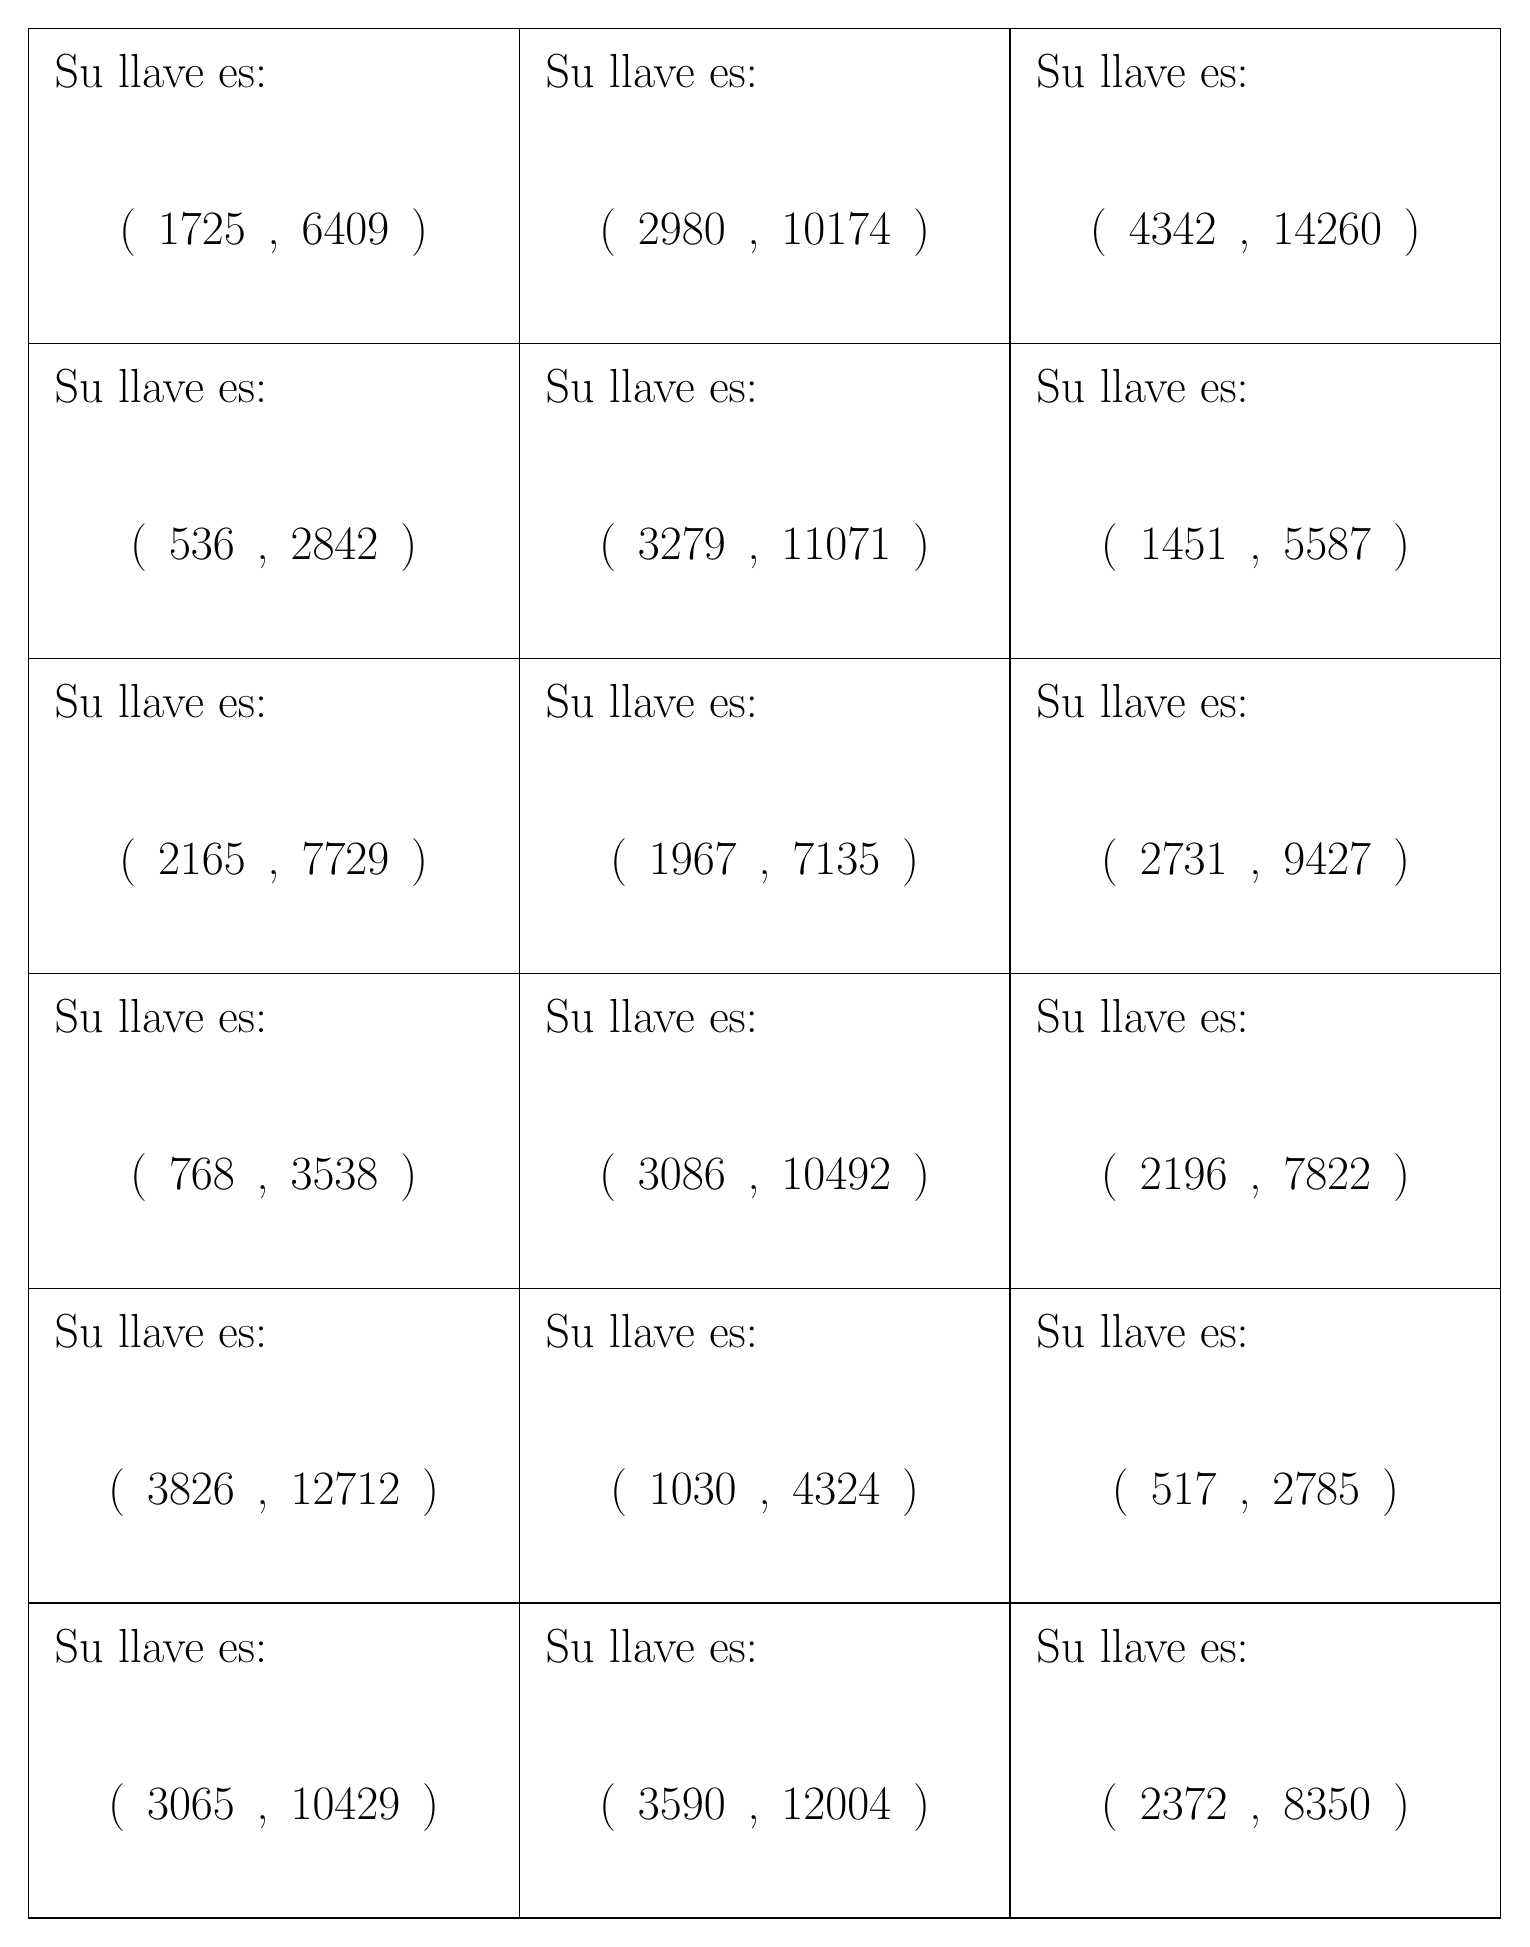
\begin{tikzpicture}
\usetikzlibrary{positioning} % for relative note placement (right = of)


\tikzset{%
    node distance=0cm,   % 0 distance between nodes so that edges coincide
    every node/.style={font=\LARGE,}, % text font size for all nodes
}

% Style of "tarjeta" node
\tikzstyle{tarjeta}=[%
    , draw                 % draw rectangle edges     
    , text width = 6cm     % min width     
    , minimum height = 4cm % min height
    , align = center       % alignment
    , outer sep = 0cm      % 0 "personal space" for nodes
    , text height=1.5cm    % vertical placement of text inside node
    , text depth=0.0cm,    % vertical placement of text inside node (modes opposite dir)
]

\def\myCols{3}
\def\myRows{6}

\newcommand{\displayPt}[2]{
    ( \,#1\, , \,#2\, )
}

% Generate first tarjeta: (tarjeta-1-1)
\pgfmathsetmacro{\myX}{int(400+4000*random())}
\pgfmathsetmacro{\myY}{int(3*\myX+1234)}
\node[tarjeta] (tarjeta-1-1) {\displayPt{\myX}{\myY}};


% Generate first column by placing nodes below (tarjeta-1-1)
\foreach \row in {2,...,\myRows}{
    \pgfmathsetmacro{\myX}{int(400+4000*random())}
    \pgfmathsetmacro{\myY}{int(3*\myX+1234)}
    \pgfmathsetmacro{\prevRow}{int(\row-1)}
    \node[tarjeta, below = of tarjeta-1-\prevRow] (tarjeta-1-\row) {\displayPt{\myX}{\myY}};
}

% Generate remaining columns by placing nodes to the right of the node in each row
\foreach \column in {2,...,\myCols}{
    \foreach \row in {1,...,\myRows}{
        \pgfmathsetmacro{\myX}{int(400+4000*random())}
        \pgfmathsetmacro{\myY}{int(3*\myX+1234)}
        \pgfmathsetmacro{\prevCol}{int(\column-1)}
        \node[tarjeta, right = of tarjeta-\prevCol-\row] (tarjeta-\column-\row) {\displayPt{\myX}{\myY}};
    }
}


% add "Su llave es:" to all tarjetas
\foreach \column in {1,...,\myCols}{
    \foreach \row in {1,...,\myRows}{
        \node[below right = 0.3cm] at (tarjeta-\column-\row.north west) {Su llave es:};
    }
}


\end{tikzpicture}
\end{document}